% nleguide.tex
% v1.0, released 31 Jan 2019
% Copyright 2019 Cambridge University Press

\documentclass{nle}
\bibliographystyle{nlelike}

\usepackage{natbib}
\usepackage{url}
\usepackage{soul}
\usepackage{algorithm}
\usepackage{algorithmic}
\urlstyle{same}
\usepackage{helvet}
\usepackage{booktabs}
\usepackage{listings}
\usepackage{xcolor}
\usepackage{amsmath,amsfonts,amsthm,amsopn}
\usepackage{epsfig}
\usepackage{graphicx}
%\usepackage{array}
\usepackage{multicol}
%\usepackage{threeparttable}
\usepackage{multirow}
\usepackage{subfigure}
\theoremstyle{definition}
\usepackage{caption2}
\newtheorem{example}{Example}


\ifpdf%
\usepackage{epstopdf}%
\else%
\fi

\newcommand{\secref}[1]{Section \ref{#1}}
\newcommand{\figref}[1]{Figure \ref{#1}}
\newcommand{\eqnref}[1]{Eq. (\ref{#1})}
\newcommand{\tabref}[1]{Table \ref{#1}}
\newcommand{\exref}[1]{Example \ref{#1}}
\newcommand{\cut}[1]{}
\newcommand{\tabincell}[2]{\begin{tabular}{@{}#1@{}}#2\end{tabular}}
\newcommand{\KZ}[1]{\textcolor{blue}{Kenny: #1}}

\begin{document}
\label{firstpage}

\lefttitle{Reduce Repetition in CNN-based Summarization}
\righttitle{Natural Language Engineering}

\papertitle{Article}

\jnlPage{1}{00}
\jnlDoiYr{2019}
\doival{10.1017/xxxxx}

\title{Reducing Repetition in Convolutional Abstractive Summarization}

\begin{authgrp}
\author{Yizhu Liu}
\affiliation{Department of Computer Science and Engineering, Shanghai Jiao Tong University, Shanghai, China \\
        \email{liuyizhu@sjtu.edu.cn}}
\author{Xinyue Chen}
\affiliation{Department of Computer Science and Engineering, Shanghai Jiao Tong University, Shanghai, China \\
        \email{sherryicss@gmail.com}}
\author{Xusheng Luo}
\affiliation{Search and Recommendation Team, Alibaba Group, Hangzhou, China \\
        \email{lxs140564@alibaba.com}}
\author{ Kenny Q. Zhu}
\affiliation{Department of Computer Science and Engineering, Shanghai Jiao Tong University, Shanghai, China \\
        \email{kzhu@cs.sjtu.edu.cn}}
\end{authgrp}

\history{(Received xx xxx xxx; revised xx xxx xxx; accepted xx xxx xxx)}
%\received{20 March 1995; revised 30 September 1998}

\begin{abstract}
Convolutional sequence to sequence (CNN seq2seq) models have met success in abstractive summarization. However, their outputs often contain repetitive word sequences and logical inconsistencies,
limiting the practicality of their application. 
In this paper, we find the reasons behind repetition problem in abstractive summarization and solve the repetition problem.
We propose to reduce the repetition in summaries by 
Attention Filter mechanism (ATTF) and Sentence-level Backtracking Decoder (SBD),
which dynamically redistributes attention over the input sequence 
as the output sentences are generated. 
The ATTF can record previously attended locations in the source document directly and prevent decoder from attending to these locations. The SBD prevents the decoder from generating similar sentences more than once via backtracking at test.
The proposed model outperforms the baselines 
in terms of ROUGE score, repeatedness, and readability. 
The results show that this approach 
generates high-quality summaries with minimal repetition,
and makes the reading experience better.
\end{abstract}

\maketitle
\section{Introduction}
\label{sec:intro}

Abstractive summarization is the task of creating a short, accurate,
informative and fluent summary from a longer text document.
It attempts to reproduce the semantics and topics of original text
by paraphrasing. 
Recently, sequence to sequence
models~\citep{RushCW15,ChopraAR16,NallapatiZSGX16,SeeLM17,PaulusXS17}
have made great progress on abstractive summarization.
Recent study~\citep{bai2018empirical} suggests that, 
without additional, complicated structures or features,
convolutional sequence to sequence 
(CNN seq2seq) models~\citep{gehring2017convs2s,FanGA18,LiuLZ18} 
are more effective and can be trained much faster due to 
its intrinsic parallel nature compared to recurrent neural networks (RNN).
Furthermore, unlike RNN-based models, 
the convolutional models have more stable gradients 
because of its backpropagation paths. 
Self-attention-based model is 
the basis of many recent state-of-the-art systems,
which always need multi-layer self-attention and have greater computational complexity than CNN seq2seq models \citep{CompareTrans}.
Thus, we take CNN seq2seq models as the target model to improve on and
compare with in this paper.

Unfortunately, just like RNN-based models, CNN-based models also produce
summaries with substantial repeated word sequences which impacts the reading efficiency.
\tabref{tab:example} illustrates one 
test case from the CNN/Daily Mail summarization dataset. 
In this case, the basic CNN produces two 
identical sentences (italized) in the result. 
Unlike machine translation or paraphrasing in which the output words
and input words are almost one-to-one aligned, the output of summarization
is ``compressed'' from the input document. Naturally, every sentence or 
word sequence in the summary corresponds to one or more places in the source
document. If there were two identical word sequences in the summary,
they might be looking at and summarizing the same ``spots'' in the source.
This is evident from the attention map for the three sentences generated by 
CNN, shown in \figref{fig:attn_map}. The 1st and 3rd sentences attend to
the same location in the source (red boxes), 
while the 2nd sentence attends to another separate location in the source (green box). 
The two attention maps in the red boxes are very similar.

\begin{table}[th!]
	\centering
	\caption{Summary generated by the basic CNN model}
	\begin{tabular}{|l|}
		\hline \bf Source Document \\
		\hline manchester city are rivalling manchester united and arsenal for valenciennes \\
		teenage defender dayot upamecano . the 16-year-old almost joined united in \\
		the january transfer window only for him to opt to stay in france for a few \\
		more months . centre-back umecano has played for france at u16 and u17 \\
		level . monaco , inter milan and paris stgermain had also expressed interest. \\
		fourth-placed city face aston villa at the etihad stadium on saturday . \\
		\hline \bf Reference summary \\
		\hline dayot upamecano was close to signing for manchester united in january . \\
		the 16-year-old, however , opted to stay in france with valenciennes . \\
		centre-back upamecano has played for france at u16 and u17 level . \\
		arsenal are also interested in the defender as man city join chase . \\
		\hline \bf Basic CNN model (CNN) \\
		\hline \textit{manchester city face aston villa at the etihad stadium on saturday .}\\
		the 16-year-old almost joined united in the january transfer window . \\
		\textit{manchester city face aston villa at the etihad stadium on saturday .}\\
		\hline
	\end{tabular}
	\label{tab:example}
\end{table}


\begin{figure}[th!]
	\centering
	\subfigure[Attention distribution]{
		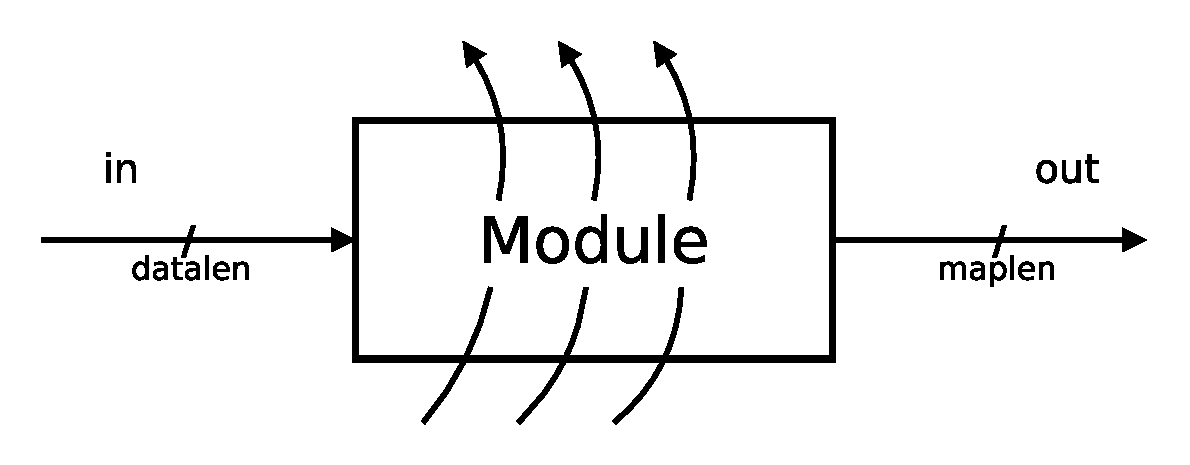
\includegraphics[width=0.8\linewidth]{map}
	}
	\quad
	\subfigure[Green box]{
		\includegraphics[width=0.44\linewidth]{map_1}
	}
	\quad
	\subfigure[Red box]{
		\includegraphics[width=0.44\linewidth]{map_2}
	}
	\caption{Attention for example on CNN model in \tabref{tab:example}}
	\label{fig:attn_map}
\end{figure}

Driven by this intuition, a few efforts have been made on ``remembering''
what has been focused on before at decoding. 
For example, 
\cite{PaulusXS17} and 
\cite{FanGA18} use intra-temporal 
attention~\citep{NallapatiZSGX16} as well as intra-decoder attention to avoid
attending to the same parts in the source by 
revising attention scores while decoding. 
\cite{SeeLM17} and \cite{GehrmannDR18}
respectively propose coverage mechanism and coverage penalty,
which records the sum of attention distributions of all previously generated words 
%to keep track of what has been summarized in different way.  
in a different way to track the summarized information.  
While these approaches discourage repetition to some extent,
they do so in an indirect manner. That is, they do not 
make use of the attention information in source directly.
Consequently, they may still generate repeated phrases, 
especially in long sentences (shown in the first 5 sections of
\tabref{tab:strong_methods}).


\begin{table}[th!]
	\begin{center}
		\caption{\label{tab:strong_methods} Generated summaries of the source in \tabref{tab:example}}
		\begin{tabular}{|l|}%{|p{7cm}|rl|}
			
			\hline \bf Intra-temporal attention (ITA) \\
			\hline \textit{manchester city face aston villa at the etihad stadium on saturday .} \\
			\textit{manchester city face aston villa at the etihad stadium on saturday .}\\
			\hline \bf Intra-temporal $+$ Intra-decoder (ITDA) \\
			\hline \textit{manchester city are rivalling manchester united and arsenal }for valenciennes\\
			teenage . manchester city face aston villa at the etihad stadium on saturday . \\
			\textit{manchester city are rivalling manchester united and arsenal }. \\
			\hline \bf Coverage model (COV) \\
			\hline \textit{manchester city face aston villa at the etihad stadium on saturday .} \\
			manchester city are rivalling manchester united and arsenal for valenciennes . \\
			\textit{manchester city face aston villa at the etihad stadium on saturday .}\\
			\hline \bf Coverage penalty (COVP)\\
			\hline \textit{manchester city face aston villa at the etihad stadium on saturday .}\\
			\textit{manchester city face aston villa at the etihad stadium on saturday .}\\
			manchester city are rivalling manchester united and arsenal .\\
			\hline \bf Semantic cohesion loss (SCL) \\
			\hline \textit{manchester city are rivalling manchester united and arsenal for } defender dayot upamecano . \\
			\textit{manchester city are rivalling for} valenciennes teenage. \\
			\hline \bf Diverse Convolutional Seq2Seq  Model (DivCNN) \\
			\hline manchester city face aston villa at the etihad stadium on saturday . \\
			\underline{the 16-year-old} has played for \underline{france}  for a few months.\\ 
			\hline \bf Trigram decoder (TRI) \\
			\hline \underline{defender dayot upamecano} has played for \underline{france} at unk and unk level .\\ 
			manchester city face aston villa at the etihad stadium on saturday . \\
			\hline \bf Ours (Attention Filter + Sentence-level Backtracking decoder) \\
			\hline manchester city face aston villa at the etihad stadium on saturday . \\
			the 16-year-old almost joined united in the january transfer window . \\
			manchester city are rivalling manchester united and arsenal for teenage defender daypot upamecano .\\
			\hline
		\end{tabular}
	\end{center}
\end{table}

In this paper, we propose an attention filter mechanism that directly 
redistributes the attention from each word in the output summary to the source. 
It does so by computing the parts of interest (POIs) in the source
per segment in the summary
and then minimizing the attention scores of
words in these POIs that have already been attended to by the preceding 
segments during decoding. 
Different segments in summary thus do not attend to the same semantic spots
of source, and repetition is reduced. 
We can get segments in different ways.
As shown in \tabref{tab:punct}, we compare the segments in different types.
The baseline with sentence as a segment (sentence-level segment) 
always loses important information in reference summary, such as ``silas randall timberlake''.
The first sentence in generated summary based on sentence-level segment attends to 
the second sentence in source. 
The attention score of second sentence in source is minimized,
and this source sentence is no longer attended. 
So, the model with sentence-level segment loses the important information ``silas randall timberlake''
during decoding.
The baseline with N-gram as a segment (N-gram segment) may bring about grammatical and semantic problems.
Suppose that $N$ equals to 3~\footnote{We set $N$ as 3 because ground-truth summaries almost never contain the same trigram twice.}, 
as shown in \tabref{tab:punct},
the green part of generated summary based N-gram segment does not attend to the ``the couple announced''
in source document. 
As N-gram cannot be seen as a complete and accurate semantic unit,
the decoder of model with N-gram segment attends to the segment in source with inaccurate grammar and semantics.
Thus, the generated summary based on N-gram segment has grammatical and semantic errors.
We use punctuations to separate the source or target into segments,
since punctuations play an important role in written language to organize
the grammatical structures and to clarify the meaning of sentences.~\citep{briscoe1996,Kim19,LiWE19}
It is very simple but effective. 
In this paper, a segment means 
a sentence or clause delimited by punctuation,
which carries syntactic and semantic information. 
Specifically, we calculate the attention in terms of segments 
(larger semantic units than tokens and smaller semantic units than sentences)
which intuitively helps with emphasis of attention and POIs in source.
This is different from previous approaches
which all do not exactly pinpoint these parts in the source,
which we believe is critical in reducing repetition. 

\begin{table}[th!]
	\begin{center}
		\caption{The summary generated by attention filter mechanism with different type of segments. 
			The parts of text in different colors denote segments. The segments in the same color attend to the same POI in the source.}
		\begin{tabular}{|l|}%{|p{7cm}|rl|}
			\hline 
			\textbf{Source} \\
			\hline 
			(1)justin timberlake and jessica biel , welcome to parenthood . \\
			(2)the celebrity couple announced the arrival of their son , silas randall timberlake, ... \\
			(3)silas was the middle name of timberlake ’s maternal grandfather bill bomar , who died in 2012 .\\
			(4)the couple announced the pregnancy in january , ... \\
			(5)it is the first baby for both .  \\
			\hline 
			\textbf{Reference} \\
			\hline 
			timberlake and jessica biel welcome son silas randall timberlake. \\
			the couple announced the pregnancy in january . \\
			\hline 
			\textbf{Sentence-level segment} \\
			\hline \textcolor{blue}{the couple announced the arrival of their son .} \\
			\textcolor{brown}{it is the first baby for both} \textcolor{black}{.}  \\
			\hline 
			\textbf{N-gram segment} \\
			\hline \textcolor{blue}{the couple announced} \textcolor{green}{silas randall timberlake} \textcolor{red}{pregnancy in january }  \textcolor{black}{.}\\
			\hline
			\textbf{Segment: a sentence or clause delimited by punctuation} \\
			\hline \textcolor{blue}{the couple announced the arrival of their son ,} \textcolor{green}{silas randall timberlake .} \\
			\textcolor{red}{the couple announced the pregnancy in january .} \\ 
			\textcolor{brown}{it is the first baby for both} \textcolor{black}{.} \\
			\hline 
		\end{tabular}
		\label{tab:punct}
	\end{center}
\end{table}

Despite the above effort, there are cases, where similar sentences 
exist in the same source document:
\begin{example}
	\label{ex:repeatsrc}
	%\fbox{
	%\parbox{0.9\columnwidth}{
	\small{``..the standout fixture in the league on saturday sees leaders 
		chelsea welcome manchester united ... chelsea midfielder oriol romeu, 
		\textbf{currently on loan at stuttgart}, ... romeu is 
		\textbf{currently on a season-long loan at bundesliga side stuttgart.}''} 
	%}}
\end{example}

In this case, even if the decoder attends to different POIs of 
source document as it produces words, repetition may still result.  
At different time steps, 
the decoder may attend 
to sentences that are similar in different positions.
One potential solution to this is semantic cohesion loss (SCL)~\citep{elikyilmazBHC18}
which takes the cosine similarity between two consecutively generated sentences
as part of the loss function. It may attend to the same POI
and generate similar sentences (SCL row in \tabref{tab:strong_methods}).  
The other is Diverse Convolutional Seq2Seq
Model (DivCNN)~\citep{DivC2C19}, 
which introduces DPPs into deep neural network (DNN) attention adjustment
and uses status of DNN as quality and diversity (QD-score) for abstractive summarization.
DivCNN first selects the attention distribution of the subsets of source with high QD-score
first and then adds it into model loss as a regularization.
DivCNN does not directly redistribut the attention,
so it may still attend to similar POIs.
In order to improve QD-score, DivCNN tends to attend to scattered subsets of sentences in source document,
which leads to semantic incoherence. 
As shown in \tabref{tab:strong_methods} (DivCNN row ),
the content about the 16-year-old 
is inconsistent with source document.
Besides, trigram decoder (TRI)~\citep{PaulusXS17} 
directly forbids repetition of previously generated trigrams at test time. 
While this simple but crude method avoids the repeat of any kind
completely, 
it ignores the fact that \textit{some amount of repetition} may exist
in natural summaries.  
On the other hand, the meddling of the beam search at runtime causes another problem: 
it tends to generate sentences that are logically incorrect. 
In \tabref{tab:strong_methods} (TRI row), the defender dayot didn't
really play for France, according to the source.
That is, the subject and object are mismatched.
As trigram cannot reflect the complete semantic information, 
trigram decoder always generates logically incorrect summaries 
due to the trigram-based meddling of beam search 
during testing. 
In order to avoid the logical incorrectness caused by trigram decoder,
we introduce  a {\em sentence-level} backtracking decoder
that prohibits the repeat of same sentence at test time. 
Compared with trigram decoder, 
sentence-level backtracking decoder can avoid repetition and generate more logical summaries. 
Our summary produced for the example is shown in last section of 
\tabref{tab:strong_methods}.

Reducing repetition in abstractive summarization provides high-quality summaries for users and improves their reading efficiency.
We expect that other natural language generation (NLG) tasks suffered from repetition problem can be enhanced with our approach. 
Our contributions are summarized as follows:
\begin{enumerate}
	\item We find the reasons behind repetition problem in abstractive summaries generated
	by CNN seq2seq models.
	\item We propose new metrics to evaluate this problem: Repeatedness and Readability.
	\item We propose an effective approach that redistributes attention scores 
	during training time, and prevents repetition by sentence backtracking
	at runtime to reduce repetition in CNN seq2seq model.
	\item Our approach
	outperforms the state-of-the-art (SOTA) repetition reduction approaches on CNN-based models
	substantially by all evaluation metrics, including ROUGE scores, 
	repeatedness and readability.
\end{enumerate}

Next, we present the basic CNN seq2seq model and our extension, 
followed by the evaluation of our approach and a discussion of related work.

\section{Approach}
\label{sec:approach}

In this section, we describe the model architecture used for our experiments
and propose our novel repetition reduction method, which is an extension to the basic model.
~\footnote{
	All of the data and source code
	can be downloaded from http://202.120.38.146/sumrep.}

In summarization task, the input (source document) and
output (summary) are both sequences of words.
Suppose the input and output are respectively represented as
$\textbf{x} = (x_{1},x_{2},...,x_{m})$ and 
$\textbf{y} = (y_{1}, y_{2},..., y_{n})$ ($m>n$),
the goal is to maximize the conditional probability
$p(\textbf{y}|\textbf{x})$:
\begin{equation}
	p(\textbf{y} | \textbf{x}) \!=\! {\prod^n_{t} {p(y_{t} | y_{1}, y_{2},..., y_{t-1}, \textbf{x}})}
\end{equation}

%Our goal is to model the above conditional probability in such a way that the 
Furthermore, we aim to generate summaries that are not only fluent 
and logically consistent with source document, but also with 
a small amount of repeatedness, which is natural in human written summaries.  
%(results illustrated in \tabref{tab:eval_repe}). 
%We aim at getting the above conditional probability which can generate summaries without repetition.

\subsection{Basic CNN seq2seq Model}
\label{sec:basic}
Our basic model is multi-layer convolutional seq2seq networks \citep{gehring2017convs2s} with attention mechanism
\footnote{\url{https://github.com/facebookresearch/fairseq-py}}, 
as illustrated in \figref{fig:basicModel}. 

\begin{figure}[th]
	\centering
	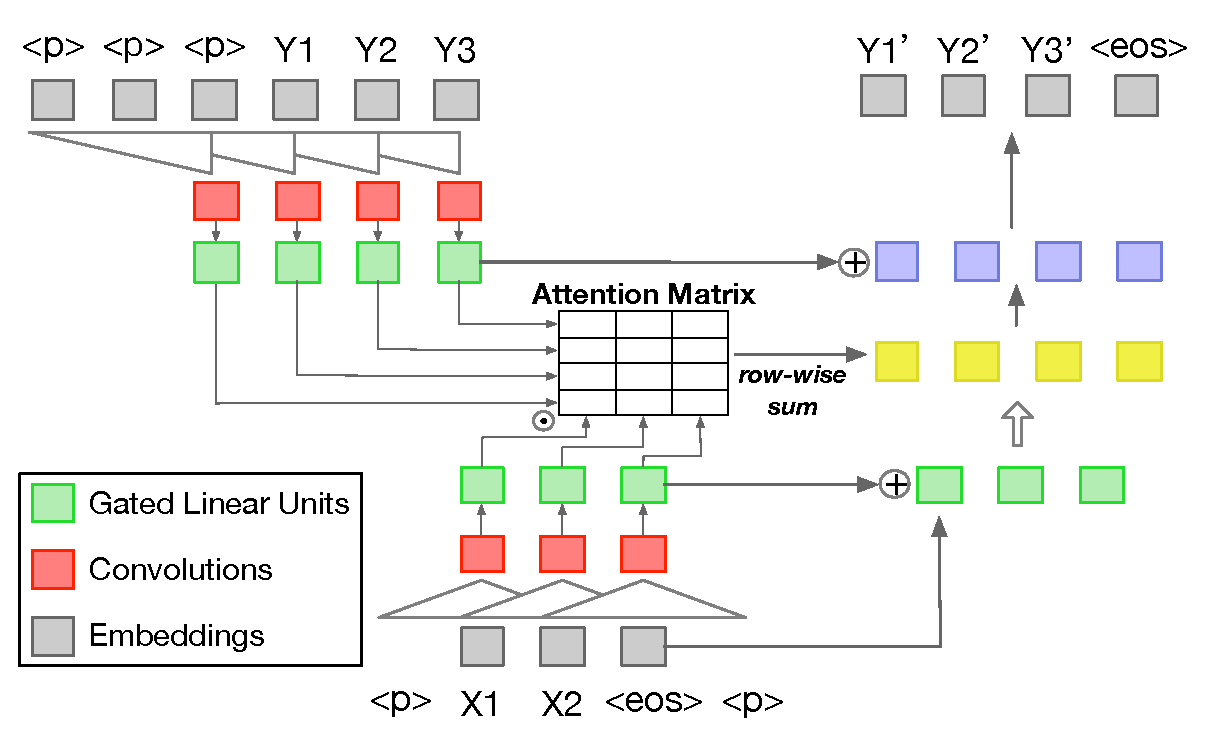
\includegraphics[width=0.8\linewidth]{cnn}
	\caption{Convolutional seq2seq model.}
	%$\odot$ stands for inner product. $\oplus$ stands for element-wise addition.}
	\label{fig:basicModel}
\end{figure}

For CNN seq2seq models, we combine word embeddings and position embeddings to obtain input $\mathbf{X} = (X_1,...,X_m)$ and output $\mathbf{Y}=(Y_1,...,Y_n)$. 
%We denote $\mathbf { z } ^ { l }$ and $\mathbf { h } ^ { l }$ 
We denote $\mathbf { z } ^ { l } = \left( z _ { 1 } ^ { l } , \ldots , z _ { m     } ^ { l } \right)$ and $\mathbf { h } ^ { l } = \left( h _ { 1 } ^ { l } , \ldots , h _ { n } ^ { l } \right)$ 
respectively as convolutional output of the encoder and
decoder in the $l$-th layer.
Each element of the output
sequence generated by the decoder network is fed
back into the next layer of decoder network.
In each layer, GLU \citep{DauphinFAG17} and residual connections \citep{HeZRS16}
are used respectively as a non-linear gate and guarantee for sufficient depth of the network.  
\begin{equation}
	h _ { i } ^ { l } = GLU \left( W ^ { l } \left[ h _ {i-k/2 } ^ { l - 1 } , \ldots , h _ { i+k/2 } ^ { l - 1 } \right] + b _ { w } ^ { l } \right) + h _ { i } ^ { l - 1 }
\end{equation} 
where \textit{k} is kernel width. $W$ and $b$ are trainable parameters.
Next, we compute the probability distribution for the next word
using the top decoder output:
\begin{equation}
	p \left( y _ { i + 1 } | y _ { 1 } , \ldots , y _ { i } , \mathbf { x } \right) = \operatorname { softmax } \left( W _ { o } h _ { i } ^ { L } + b _ { o } \right)
\end{equation}

For each decoder layer, the multi-step attention integrates encoder information. 
We compute decoder state $d_{i}^{l}$ for attention via
\begin{equation}
	d _ { i } ^ { l } = W _ { d } ^ { l } h _ { i } ^ { l } + b _ { d } ^ { l } + Y _ { i }
\end{equation}

\begin{equation}\label{eq:a}
	a _ { i j } ^ { l } = \frac { \exp \left( d _ { i } ^ { l } \cdot z _ { j } ^ { u } \right) } { \sum _ { t = 1 } ^ { m } \exp \left( d _ { i } ^ { l } \cdot z _ { t } ^ { u } \right) }
\end{equation}
\begin{equation}\label{eq:c}
	c _ { i } ^ { l } = \sum _ { j = 1 } ^ { m } a _ { i j } ^ { l } \left( z _ { j } ^ { u } + X_j \right)
\end{equation}
where $d_{i}^{l}$ is decoder state, $z_{j}^{u}$ is the encoder state, 
$u$ is the last layer of encoder
and $a_{ij}$ is attention score.
The inner product between decoder state and encoder outputs is used 
to measure the affinity. 
The conditional input to the current 
decoder layer is a weighted sum of encoder states and input representations.
Finally, $c _ { i } ^ { l }$ is added to $h_{i}^{l}$, which forms the input for the next decoder layer or the final output.

\subsection{Attention Filter Mechanism (ATTF)}
\label{sec:attf}

\begin{figure}[th]
	\centering
	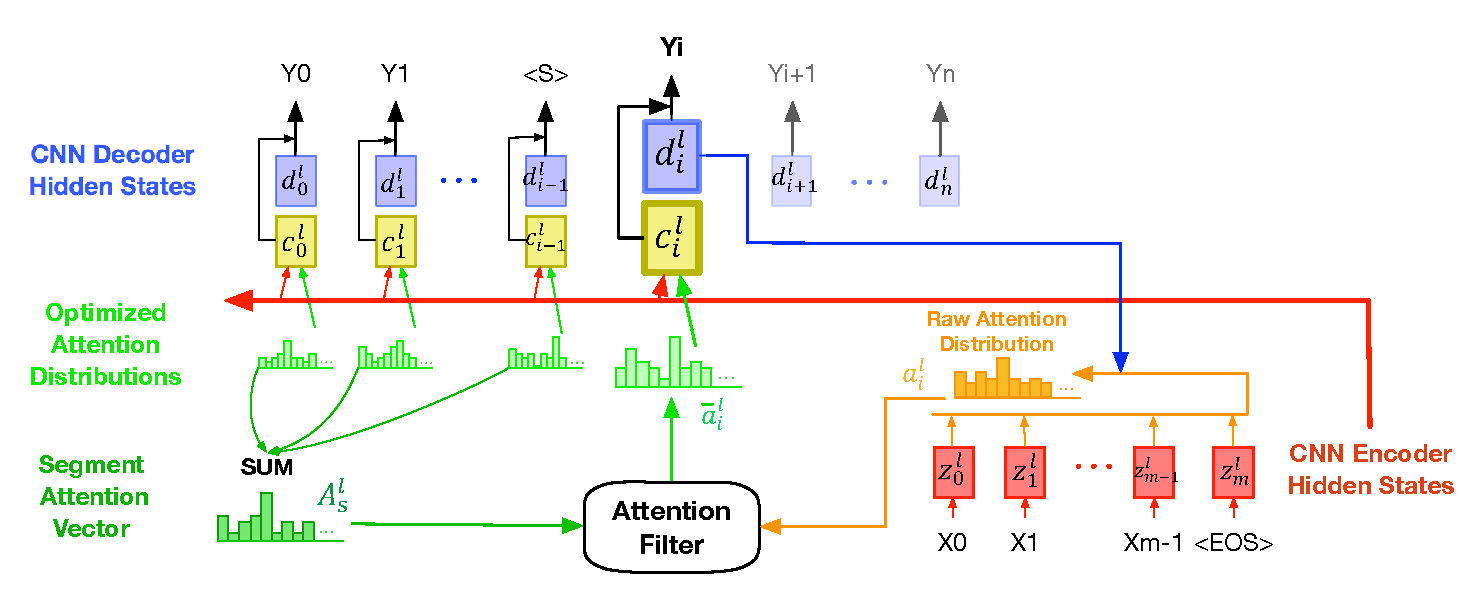
\epsfig{file=model.eps, width=1.0\columnwidth}
	\caption{Overview of Attention Filter Mechanism (ATTF)}
	\label{fig:model_main}
\end{figure}


\label{sec:attnf}
We propose an attention filter mechanism as a novel extension 
to the basic model,
which can record previously attended locations 
in the source document directly and generate summaries 
with a natural level of repeatedness. 
This method aims at relieving the repetition problem caused by 
decoders attending to the same POI in source document.

In this mechanism, both source document and summary are 
respectively split into 
\textit{sections} and \textit{segments} by punctuations. We
denote the punctuation marks as \verb#<S>#.
$\mathbf{u}=(u_{0},u_{1},...,u_{M})$ 
and $\mathbf{v}=(v_{0},v_{1},...,v_{N})$
denote the positions of \verb#<S># in source document and summary.
Both $u_{0}$ and $v_{0}$ are $-1$.
Therefore, we can represent source document as $\mathbf{U}=(U_{0},U_{1},...,U_{M-1})$ in the form of \textit{sections}. Similarly, for summaries, we have $\mathbf{V}=(V_{0},V_{1},...,V_{N-1})$. 
$U_i$ and $V_i$ are
both sequence of tokens minus the punctuation tokens.

Let $D$ denote the number of tokens in the source document.
We define \textit{segment attention vector} in the $l$-th layer as 
$A^{l} = (A_{0}^{l}, A_{1}^{l},..., A_{N}^{l})$, 
where $A_s^l\subset \mathbb{R}^{D}$ is a vector representing 
segment attention distribution, of the $s$-th \textit{segment},
over tokens in the source document. Summing up attention score vectors 
of each position in the $s$-th \textit{segment}:
%which is the sum of attention distributions over each section in summary:

\begin{equation}
	A_{s}^{l} = \sum_{i=v_{s-1}+1}^{v_{s}-1}a_{i}^{l}
\end{equation}
where $a_i^l$ is also a $D$-dimensional vector that records 
the attention scores of the $i$-th token in the summary over 
tokens in the source document. In other words, $ A_{s}^{l}$ 
measures the relevance between tokens of the source document and 
the $s$-th \textit{segment} $V_s$. 
We set $A_{0}^{l}$ as zero vector, because nothing is attended before generating 
the first \textit{segment}. 


To find the most attended \textit{sections}, 
we sort the elements inside the filter vector, 
$A_{s}^{l}$, in descending order, 
and record the top $k$ elements' positions in 
the source document as: 
\begin{equation}
	\mathbf{p}=(p_{0},...,p_{k})
\end{equation}
where $k=v_{s}-v_{s-1}-1$. 
$k$ is the same as the number of tokens in the $s$-th \textit{segment},
because each token in a \textit{segment} is aligned with at least one token in source document, according to the principle of the seq2seq model.
Thus, for the $s$-th \textit{segment}, 
we observe top $k$ most attended tokens in source document to find the most attended \textit{sections}.
Next, we locate these elements in the source document as well as
the \textit{sections} they belong to. 
We assign each section a set of positions that have been attended to, 
$P_{U_{t}}$. 
If the size of $P_{U_{t}}$ is larger than
$\beta$, a predefined constant,
the \textit{section} $U_{t}$ should not be attended again. 
That is, $U_{t}$ is a POI of segment $V_{s}$.
$\mathbb{U}_{s}$ denotes a set of all such POIs for $V_s$.
$\mathbb{U}_{0}$ is an empty set.

We construct two multi-hot vectors $g_{s}$ and $g'_{s}$ for each \textit{segment} $V_{s}$.
The dimensions of them are the
same as $A_{s}^{l}$. For $g_{s}$, we set elements on the position of tokens
belonging to sections in $\mathbb{U}_{s}$ to 0, and other
positions to 1. 
$g'_{sj}$ denotes $j$-th element of $g'_{s}$, which is the flipped version of $\prod \limits_{q=0}^{s}g_{qj}$. 
The filter on $a_{ij}^{l}$ in Equation (\ref{eq:a}) is given as:
\begin{equation}
	\tilde{a}_{ij}^{l} = a_{ij}^{l}\prod_{q=0}^{s}g_{qj} + \min \limits_{A_{s}}\left(\frac{A_{sj}^{l}}{v_{s}-v_{s-1}-1}\right)g_{sj}'
\end{equation}
where $v_{s}$ is the maximum value in 
$\mathbf{v}$ that is smaller than $i$,  and $\tilde{a}_{ij}^l$ is the filtered
attention score. $A_{sj}$ is the attention score between $j$-th token
of the source document and the $s$-th \textit{segment}. 
$g_{sj}$ and $g_{sj}'$ denote whether $j$-th token
of the source document has been attended.
When $\prod \limits_{q=0}^{s}g_{qj}$ is zero, $g_{sj}'$ is $1$.
This means that the $j$-th token of the source document has been attended before.
We penalize the attention score of attended tokens in source document
We take the minimum attention score between tokens in source document and summary 
(i.e. $\min \limits_{A_{s}}\left(\frac{A_{sj}^{l}}{v_{s}-v_{s-1}-1}\right)$ )
as the attention score between the $i$-th token in target and the $j$-th token in source.
Equation (\ref{eq:c}) now becomes:
\begin{equation}
	c _ { i } ^ { l } = \sum _ { j = 1 } ^ { m } \tilde{a}_{ij}^{l} \left( z _ { j } ^ { u } + X_j \right)
\end{equation}

By using segment-wise attention and revising attention scores of attended POIs directly,
our model optimizes the
attention distribution between encoder states and decoder states in such a way that
the alignment relationship between source document and summary is enhanced, 
and noise for attention from encoder outputs is reduced. 
As shown in \tabref{tab:attn_exp}, the segments in example are separated by punctuation.
For basic CNN model, the 2nd and 3rd sentence repeatedly attend to 
the 5th segment in source.
After applying ATTF model, 
the attention score of 3rd and 5th segment in source are penalized 
during generating words in 3rd sentence of ATTF.
The last sentence of the summary generated by ATTF attend to 7th segment in source.

\begin{table}[th!]
	\begin{center}
		\caption{\label{tab:attn_exp} Summary generated by the basic CNN model and ATTF model}
		\begin{tabular}{|l|l|}%{|p{7cm}|rl|}
			\hline 
			\multicolumn{2}{|c|}{\bf Source document} \\
			\hline
			\multicolumn{2}{|c|}{\tabincell{l}{(1)justin timberlake and jessica biel, (2)welcome to parenthood. 
					(3)the celebrity couple announced the arrival \\
					of their son, 
					(4)... 
					(5)the couple announced the pregnancy in january, (6)...  
					(7)it is the first baby for both . }} \\
			\hline 
			\bf Basic CNN model (CNN) & \bf ATTF (our) \\
			\hline 
			\tabincell{l}{(1)the couple announced the the arrival of their son. \\
				(2)the couple announced the pregnancy in january. \\ 
				(3)the couple announced the pregnancy in january. } 
			& \tabincell{l}{(1)the couple announced the arrival of their son. \\
				(2)the couple announced the pregnancy in january. \\
				(3)it is the first baby for both. } \\
			\hline
		\end{tabular}
	\end{center}
\end{table}
The attention filter mechanism helps avoid repeatedly attending to the same POIs, and therefore avoid repetition in summary generation.


\subsection{Sentence-level Backtracking Decoder (SBD)}
\label{sec:sbd}

To tackle repeated sentences or phrases in the source (\exref{ex:repeatsrc}), 
we propose a sentence-level backtracking decoder.

\begin{figure}[th]
	\centering
	\includegraphics[width=0.8\linewidth]{SBD}
	\caption{Backtracking in Beam Search ($b=3$). 
		This figure shows the progress of generating summary at test. The circles denote the
		candidate words (choices) in vocabulary, 
		which are sorted by the probability of being selected in
		descending order. Each circle at level $l$ has $N$ choices 
		at level $l+1$. $N$ is the number of words in vocabulary. 
		The number in circles is the order of these choices according to the
		probability. The generation order is from level 1 (top) to level 3 (bottom).}
	\label{fig:beam}
\end{figure}

At test time, we prevent the decoder from generating identical or
very similar sentences more than once via backtracking. 
An intuitive solution is to backtrack the generation process to the beginning
of the repeated segment, and regenerate it by following the second best choice
in the beam. We call this simple approach \textbf{SBD-b1}.
However, this is sub-optimal
because the parents of the current top $b$ choices may not include all the top $b$ choices at the
parent level. Here $b$ is the beam size. As shown in \figref{fig:beam}, suppose that level 3 is the
beginning of the repeated segment, the first choices at level 1 and 2 are excluded by beam search. 

An alternative approach (\textbf{SBD-b2}) backtracks all the way until the current
top $b$ choices all share the same prefix token sequence. This means
that the current best choices in the beam reach some consensus that
the generated prefix summary is good and should be retained. 
While this algorithm backtracks further and may
include better choices, it does not completely solve the problem of SBD-b1. 
As shown in \figref{fig:beam}, 
suppose that level 3 is the beginning of the repeated segment and the second choices in
level 1 is the only prefix token sequence of top $b$ choices in level 2, the first and third choices at
level 1 are excluded by beam search after generating words based on second choice in level 1.

\begin{table}[th!]
	\begin{center}
		\caption{\label{tab:sbd_exp} Summary generated by basic CNN model with different backtracking methods.}
		\begin{tabular}{|l|l|}%{|p{7cm}|rl|}
			\hline 
			\multicolumn{2}{|c|}{\bf Source document} \\
			\hline
			\multicolumn{2}{|c|}{\tabincell{l}{
					justin timberlake and jessica biel , welcome to parenthood . the celebrity couple announced \\
					the arrival of their son , silas randall timberlake ,... `` silas was the middle name of \\
					timberlake 's maternal grandfather bill bomar , who died in 2012 ,... the couple announced \\
					the pregnancy in january , with an instagram post . it is the first baby for both .
			}} \\
			\hline 
			\bf Basic CNN model (CNN)
			& \tabincell{l}{
				the couple announced the arrival of their son. \\
				the couple announced the pregnancy in january. \\
				\textit{the couple announced the pregnancy in january. (repeated segment)} \\
			} \\
			\hline 
			\bf CNN+TRI
			& \tabincell{l}{
				the couple announced the arrival of their son. \\
				\underline{silas randall timberlake , who died in 2012.} \\
			} \\
			\hline
			\bf CNN+SBD-b1
			& \tabincell{l}{
				the couple announced the arrival of their son. \\
				the couple announced the pregnancy in january. \\
				\underline{silas was the middle name of timberlake 's maternal grandfather.} \\
			} \\
			\hline
			\bf CNN+SBD-b2
			& \tabincell{l}{
				the couple announced the arrival of their son. \\
				\underline{silas randall timberlake , died in 2012.} \\
			} \\
			\hline
			\bf CNN+SBD
			& \tabincell{l}{
				the couple announced the arrival of their son. \\
				they announced the pregnancy in january, with an instagram post. \\
			} \\
			\hline
		\end{tabular}
	\end{center}
\end{table}

Our best approach (\textbf{SBD}) backtracks to the beginning of the whole summary
and regenerates all the choices in the beam up to the point before
the repeated segment. That way, all the best choices are known to the
algorithm and we can make an optimal choice after excluding the first word
of the previously repeated segment. 
As shown in \tabref{tab:sbd_exp},
SBD-b1 and SBD-b2 backtrack the generator process
to ``january.'' and ``son.'' respectively.
The summaries generated by SBD-b1 and SBD-b2 
are incoherence and inconsistent with the source document.
Our best approach (SBD) will save the sequence before repeated segment, i.e., 
`\textit{
	the couple announced the arrival of their son.
	the couple announced the pregnancy in january.}
'
and backtrack to the beginning of the summary and regenerate the summary. 
When the saved sequence appears in the beam, we remove the first word (``the'') in 
repeated segment from the choices vocabulary. 
Compared with SBD-b1 and SBD-b2, SBD generates more fluent and coherence summaries.


To determine whether two sentences, 
$p$ and $q$, are similar, we define a boolean function as:
\begin{equation}\label{eq:s}
	sim(p,q) = 
	\begin{cases}
		1 &\mbox{if $o(p,q) > n\text{ OR }o(p,q) > \frac{1}{2}\cdot l$}\\
		0 &\mbox{others}
	\end{cases}
\end{equation}
where $o(p,q)$ denotes the length of 
the longest common substring (LCS) between $p$ and $q$, 
$l$ is the minimum of the lengths of $p$ and $q$, and $n$ is a constant. 
$sim(p,q)=1$ means the two sentence are similar.

This method cooperates with ATTF in 
reducing repetition caused by the noises in dataset.
Compared with \textbf{TRI},  SBD does not interrupt the beam search process in the middle of a sentence, hence significantly reducing related grammatical and factual errors. 
As shown in \tabref{tab:sbd_exp}, 
the summary generated by SBD is grammatical and factual. 
Besides, SBD is capable of producing a more informative summary since it yields more chances to other candidate sentences.

\section{Evaluation}
\label{sec:eval}
In this section, we introduce the experimental setup
and analyze the performance of different models.

\subsection{Datasets}
CNN/Daily Mail~\citep{HermannKGEKSB15}
\footnote{\url{https://cs.nyu.edu/~kcho/DMQA/}} 
is a popular summarization dataset, 
which contains news articles paired with summaries.
There are 286,817 training pairs,
13,368 validation pairs and 11,487 test pairs.
\tabref{tab:example} shows an example pair from training data.
We follow \cite{SeeLM17} in data preprocessing and use 
the non-anonymized version, which fills in the blanks with answer named entities.

Also we tried our model on other two abstractive summarization datasets about news, which are Newsroom \citep{Newsroom18} and DUC 2002 \footnote{https://www-nlpir.nist.gov/projects/duc/guidelines/2002.html}. For Newsroom, there are 1,321,995 document-summary pairs, which are divided into training (76\%), development (8\%), test (8\%), and unreleased test (8\%). At testing, we use 8\% released test data. DUC-2002 (DUC) is a test set of document-summary pairs. We use the models trained on CNN/Daily Mail to do the test on DUC and demonstrate the generalization of the models.


\subsection{Model Parameters and Evaluation Metrics}
\label{sec:expset}
In the following experiments, 
we tokenize source documents and targets 
using the word tokenization method from NLTK (Natural Language Toolkit). 
The NLTK module is a massive toolkit, 
aimed at helping with the entire Natural Language Processing (NLP) methodology.
All the competing models contain $8$ convolutional layers in
both encoders and decoders, with kernel width of $3$.
For each convolutional layer, 
we set the hidden state size to $512$ and the embedding size to $256$.
To alleviate overfitting,
we apply a \textit{dropout} ($p=0.2$) layer to 
all convolutional and fully connected layers.
Similar to \citep{gehring2017convs2s},we use Nesterov's
accelerated gradient method \citep{SutskeverMDH13} with gradient clipping $0.1$ \citep{PascanuMB13}, momentum $0.99$,
and initial learning rate $0.2$.
Training terminates when learning rate $\le 10e$-$5$.
Beam size $b=5$ at test time.

We set the threshold $\beta$ to $3$, 
because nearly $90\%$ 
of sections are with length$>=$3.
We set $n$ (Equation (\ref{eq:s})) to $5$,
since less than $5\%$ of reference summaries have
the LCS of less than $5$.
We use the following evaluation metrics:
\itemsep0em
\begin{itemize}
	
	\item \textbf{ROUGE} scores (F1), including ROUGE-1 (R-1), ROUGE-2 (R-2) and
	ROUGE-L(R-L)~\citep{rouge-a-package-for-automatic-evaluation-of-summaries}.
	ROUGE-1 and ROUGE-2 respectively refer to the overlap of unigram (each word) and bigrams between the generated summaries and reference summaries.
	ROUGE-L denotes Longest Common Subsequence (LCS) based statistics.
	ROUGE-2 is the most popular metric for summarization.
	
	\item \textbf{Repeatedness} (Rep) 
	includes N-gram repeatedness, sentence repeatedness
	and total repeatedness.
	\begin{itemize}
		\item[-] \textbf{N-gram repeatedness} is the percentage of repeated N-grams 
		in a summary:
		
		\begin{equation}
			Rep_{ngram} = \frac{n_{ngram}}{N_{ngram}}
		\end{equation}
		where $n_{ngram}$ is the number of repeated N-grams, 
		$N_{ngram}$ is the total number of N-grams in a summary.
		\item[-] \textbf{Sentence repeatedness} is the percentage of repeated 
		sentences in a summary:
		\begin{equation}
			Rep_{sent} = \frac{n_{sent}}{N_{sent}}
		\end{equation}
		where $n_{sent}$ is the number of repeated sentences, 
		$N_{sent}$ is the total number of sentences in a summary.
		For sentence repeatedness, if the sentences contain the same trigram,
		these sentence are repetitve sentences.
		\footnote{
			Any two sentences in one reference summary almost never contain 
			the same trigram \citep{PaulusXS17}.}
		\item[-] 
		\textbf{Total repeatedness} (Algorithm \ref{alg:red}) is a comprehensive score
		that unifies word-level and sentence-level repeatedness.
		It is not computed by N-gram repeatedness score 
		and sentence repeatedness score.
		
		\begin{algorithm}[th]
			\caption{Calculation of Total Repeatedness}
			\label{alg:red}
			\textbf{Input}: a sentence set $s = {s_{1}, s_{2},...,s_{n}}$\\
			%\textbf{Parameter}: Optional list of parameters\\
			\textbf{Output}: Total repeatedness percentage $p$
			\begin{algorithmic}[1] %[1] enables line numbers
				\STATE Let $total$ be the sum of lengths of the sentences in $s$.
				\STATE $n \leftarrow total$
				\STATE $overlap \leftarrow 0$
				\WHILE{$n \geq 3$}
				\STATE The lengths of LCS between two sentences from $s$ comprise a length set $L$.
				\STATE $n \leftarrow \max(L)$.
				\STATE Find a substring $b$ with length $n$ that appears most frequently in $s$.
				\STATE Let $k$ be the frequency that $b$ appears in $s$.
				\STATE $overlap \leftarrow overlap + k\cdot n$
				\STATE Remove every appearance of substring $b$ from sentences in $s$.
				\ENDWHILE
				\STATE $p \leftarrow overlap/total$
				\STATE \textbf{return $p$} 
			\end{algorithmic}
		\end{algorithm}
	\end{itemize}
	
	\item \textbf{Repeatedness Correlation} 
	measures how well 
	the total repeatedness scores of summaries generated by each model
	correlate with total repeatedness scores of reference summaries. 
	The more correlative generated summary and reference summary are,
	the better generated summary is.
	The correlation is evaluated with a set of
	three metrics, including Pearson correlation (r),
	Spearman rank coefficient ($\rho$), and Kendall's tau coefficient ($\tau$).
	Given total repeatedness scores of reference summaries (ref) and 
	their corresponding generated summaries (gen),
	$X=score(ref)=(x_1, x_2,..., x_n)$ and 
	$Y=score(gen)=(y_1, y_2,..., y_n)$, 
	we can get paired data $(X,Y)={(x_1, y_1), (x_2, y_2),..., (x_n, y_n)}$.
	$n$ is the number of pairs.
	\begin{itemize}	
		\item[-] For Pearson correlation (r),
		\begin{equation}
			r = \frac{\sum_{i=1}^{n}(x_i - \overline{X})(y_i - \overline{Y})}
			{\sqrt{\sum_{i=1}^{n}(x_i - \overline{X})^{2}\cdot\sum_{i=1}^{n}(y_i - \overline{Y})^{2}}}
		\end{equation}
		where $\overline{X}$ and $\overline{Y}$ are the mean of variables of $X$ and $Y$.
		
		\item[-] For Spearman rank coefficient,
		\begin{equation}
			\rho = \frac{\sum_{i=1}^{n}(R(x_i) - \overline{R(X)})(R(y_i) - \overline{R(Y)})}
			{\sqrt{\sum_{i=1}^{n}(R(x_i) - \overline{R(X)})^{2}
					\cdot\sum_{i=1}^{n}(R(y_i)-\overline{R(Y)})^{2}}}
		\end{equation}
		where $R(x_i)$ and $R(y_i)$ are the rank of $x_i$ and $y_i$.
		$\overline{R(X)}$ and $\overline{R(Y)}$ are the mean rank of $X$ and $Y$.
		
		\item[-] For kendall's tau coefficient,
		\begin{equation}
			\tau = \frac{n_c - n_d}{n_c + n_d} = \frac{n_c - n_d}{n(n-1)/2}
		\end{equation}
		where $n_c$ is the number of \textit{concordant} pairs.
		$n_d$ is the number of \textit{discordant} pairs.
		Any pair of total repeatedness scores $(x_{i},y_{i})$ and $(x_{j},y_{j})$, where $i<j$.
		They are said to be \textit{concordant},
		if both $x_{i}>x_{j}$ and $y_{i}>y_{j}$; or if both $x_{i}<x_{j}$ and $y_{i}<y_{j}$.
		They are said to be discordant, if $x_{i}>x_{j}$ and $y_{i}<y_{j}$; 
		or if $x_{i}<x_{j}$ and $y_{i}>y_{j}$. 
		If $x_{i}=x_{j}$ or $y_{i}=y_{j}$, the pair is neither concordant nor discordant.
	\end{itemize}
	
	
	\item \textbf{Readability} (Readable) is a human evaluation. 
	We educate human annotators to assess each summary
	from three independent perspectives: 
	\begin{itemize}
		\item[-]
		(1) Informative: How informative the summary is? 
		Is the summary logically consistent with source document? 
		\item[-]
		(2) Coherent: How coherent (between sentences) the summary is? 
		\item[-]
		(3) Fluent: How grammatical the sentences of a summary are? 
		\item[-]
		(4) Factual: Are there any factual errors in the summary?
	\end{itemize}
	Readability score will be judged on the following 5-point scale:
	Very Poor (1.0), Poor (2.0), Barely Acceptable (3.0), Good (4.0) and Very Good (5.0).
	The score reflects the fluency and readability of the summary.
\end{itemize}

We use \textit{readability} to complement ROUGE scores 
since \cite{YaoWX17} showed that the standard 
ROUGE scores cannot capture grammatical or factual errors. 
We randomly sample 300 summaries generated by each model
and manually check their readability. 
Each summary is scored by four judges proficient in English. 
The Cohen's Kappa coefficient between them is $0.66$, 
indicating agreement. Here we use the average annotation score.

\subsection{Baselines}
Our goal is to evaluate the
effectiveness of our repetition reduction technique.
We choose to implement 
all existing repetition reduction techniques on top of vanilla CNN seq2seq model.
Because the vanilla CNN seq2seq model is fast and enjoys the best accuracy among
the other vanilla RNN seq2seq models such as 
RNN seq2seq model and LSTM seq2seq model.~\citep{bai2018empirical,gehring2017convs2s}.
The vanilla CNN seq2seq model and vanilla self-attention-based model have the similar
feature capture capabilities.
With long inputs, the self-attention-based models
will have greater computational complexity~\citep{CompareTrans}, such as Transformer. 
As the inputs of summarization is very long, the self-attention-based models
always need much more time during training and testing.
Besides, the self-attention-based models contain more training parameters,
which need the memory usage at training and testing time. 

\begin{table}[th!]
	\begin{center}
		\caption{Example of generated summaries}
		\subtable[Source document and reference summary]{
			\label{tab:a}
			\begin{tabular}{|l|}%{|p{7cm}|rl|}
				\hline 
				\textbf{Source} \\
				\hline 
				justin timberlake and jessica biel, welcome to parenthood. \\
				the celebrity couple announced the arrival of their son, silas randall timberlake, ... \\
				the couple announced the pregnancy in january, ... it is the first baby for both .  \\
				\hline 
				\textbf{Reference} \\
				\hline 
				timberlake and jessica biel welcome son silas randall timberlake. \\
				the couple announced the pregnancy in january . \\
				\hline
			\end{tabular}
		}
		\qquad
		\subtable[The generaged summaries of source in (a) and their ROUGE scores]{
			\label{tab:b}
			\begin{tabular}{|c|l|c|}%{|p{7cm}|rl|}
				\hline \bf model & \bf summary & \bf R-2 \\
				\hline \textbf{COV} & \tabincell{l}{timberlake and jessica biel announced the pregnancy in january. \\
					the couple announced the pregnancy in january.} & 0.60 \\
				\hline \textbf{ATTF+SBD} & \tabincell{l}{the couple announced the arrival of their son, silas randall timberlake. \\
					the couple announced the pregnancy in january. \\ it is the first baby for both.} & 0.52 \\
				\hline
			\end{tabular}
		}
		\label{tab:compete_exp}
	\end{center}
\end{table}

We did not implement the repetition reduction methods 
on top of the seq2seq models with higher ROUGE scores,
because the effectiveness of the repetition reduction is not necessarily
reflected in the ROUGE~\citep{SeeLM17, PaulusXS17, FanGA18}.
As shown in \tabref{tab:compete_exp}, 
after reducing repetition, the summary becomes better
but the ROUGE score is not improved. 
Therefore our evaluation mainly compares
the effectiveness of different repetition reduction techniques
in terms of all four metrics above.
As we known, ROUGE is not very good at evaluating abstractive summarization
and the room for improvement on the ROUGE scores are very limited.
If the repetition reduction methods 
were applied on top of the models with higher ROUGE scores, 
the differences in ROUGE scores by these repetition reduction techniques will be
indistinguishable and complicate the analysis. 
Hence, in this work, 
we construct seven baselines 
%(\tabref{tab:baselines})
by converting
repetition reduction techniques developed on RNN seq2seq models to their
counterparts on vanilla CNN seq2seq models,
to be fair.
The baselines are as follows:
\itemsep0em
\begin{itemize}
	\item \textbf{CNN} is the original convolutional seq2seq model \citep{gehring2017convs2s}. 
	\item \textbf{ITA} integrates \textit{intra-temporal attention} \citep{NallapatiZSGX16} in CNN seq2seq model, which normalizes attention values using attention history through time stamps. 
	\item \textbf{ITDA} adds \textit{intra-decoder attention} mechanism \citep{PaulusXS17} based on ITA,
	which also normalizes attention values using past decoders states.
	It is transferred to CNN seq2seq model in \citep{FanGA18}.
	\item \textbf{COV} adopts the coverage mechanism \citep{SeeLM17}, where repeatedly
	attending to the same locations is penalized in the form of \textit{coverage loss}. 
	\item \textbf{COVP} adds the coverage penalty \citep{GehrmannDR18} to loss function,
	which increases whenever the decoder repeatedly attend to the same locations of source document.
	\item \textbf{SCL} adds semantic cohesion loss \citep{elikyilmazBHC18} to loss function.
	Semantic cohesion loss is the cosine similarity between two consecutive sentences.
	\item \textbf{DivCNN} uses Determinantal Point Processes methods(Micro DPPs and
	Macro DPPs) to produce attention distribution \citep{DivC2C19}. DPPs consider both quality and diversity, which helps model attend to different subsequence in source document.
	\item \textbf{TRI} uses \textit{trigram decoder} \citep{PaulusXS17} at testing. The generation of repetitive trigrams is banned during beam search.
\end{itemize}

\subsection{Results}
\label{sec:result}

\textbf{Accuracy.} As shown in \tabref{tab:eval_main}, 
our model (ATTF+SBD) outperforms all the baselines in ROUGE scores, 
indicating we are able to generate more
accurate summaries. 

\begin{table}[th!]
	\begin{center}
		\caption{ROUGE scores on CNN/Daily Mail dataset.}
		\subtable[The models without operations at test.]{
			\begin{tabular}{|l|c|c|c|}
				\hline
				Model &   R-1 & R-2 & R-L \\
				\hline
				CNN &  34.33 & 14.25 & 35.68 \\
				ITA &  34.30 & 14.20 & 35.67 \\
				ITDA & 34.62 & 14.52 &  35.94 \\
				COV	& 35.85 & 14.81 &  35.96 \\
				COVP & 34.53 & 14.41 &  35.81 \\
				SCL	& 35.13 & 14.61 & 35.93 \\
				DivCNN	& 35.64 & 15.01 & 35.84 \\
				ATTF & \bf 36.32 & \bf 15.38 & \bf 36.09 \\
				\hline
			\end{tabular}
		}
		\qquad
		\subtable[The models with operations at test.]{
			%\begin{tabular}{lcccccccc}
			\begin{tabular}{|l|c|c|c|}
				\hline
				Model &   R-1 & R-2 & R-L \\
				\hline
				SBD-b1* & 34.24 & 14.33 & 34.75 \\
				SBD-b2* & 35.88 & 14.83 & 35.15 \\
				SBD* & 37.19 & 15.45 & 36.03 \\
				TRI* & 36.81 & 15.47 & 36.00 \\
				ATTF+TRI* & 37.33 & 16.65 & 36.30 \\
				ATTF+SBD* & \bf 37.69 & \bf 17.02 & \bf 36.47 \\
				\hline
			\end{tabular}
		}
		\label{tab:eval_main}
	\end{center}
\end{table}


Without any special operations at testing, 
our ATTF model achieves the highest score on ROUGE, showing
its effectiveness in improving summary quality.
Models with SBD or TRI at testing
are more effective than the basic CNN seq2seq model,
because more information is involved in summary generation 
as a by-product of repetition reduction.
Compared with its two variants, SBD is a little slower 
but has higher ROUGE scores, reflecting its advantage due to
better choices taken globally.
Therefore, 
we use SBD as our backtracking decoder in the following experiments. 
The number of explored candidate hypothesis, up to a point of
repetition, is less than 30 tokens.
The ROUGE score of SBD is higher than TRI on R-1 and R-L, but lower on R-2. 
The reason is that R-2 and R-L respectively evaluate
bigram-overlap and longest common sequence between the reference
summary and generated summary. This is in line with different techniques 
in SBD and TRI, the former promoting the diversity of sentences and 
the latter promoting that of trigrams.
SBD has higher ROUGE scores than ATTF, 
because the summaries from
SBD do not have the repetition caused by attending to similar sentences in source.
Unlike ATTF, 
SBD cannot obtain the ability to attend to different POIs through training.
In \tabref{tab:src_rep}, the sentences in SBD are not repetitive, 
but summarized from the same POI.
The summaries may lose important information when only using SBD.
The readability score of SBD is lower than ATTF in \tabref{tab:eval_repe}.

\begin{table}[th!]
	\begin{center}
		\caption{Repeatedness scores (\%) and Readability scores on CNN/Daily Mail dataset.
			The ``Gold'' denotes reference summaries, which are the most readable.By default, the readability score of reference summaries is judged to be 5.0.
		}
		\subtable[The models without operations at test.]{
			\begin{tabular}{|c|c|cccccccc|}
				\hline
				& Gold & CNN  & ITA & ITDA & COV & COVP & SCL & DivCNN & ATTF \\
				\hline
				1-gram & 33.79 & 56.25 & 54.44 & 51.18 & 42.18 & 52.46 & 52.23 & 38.43 & \bf 34.98 \\
				2-gram & 2.98 & 36.55 & 34.76 & 30.64 & 16.77 & 32.11 & 34.08 & 12.62 &\bf 8.16 \\
				3-gram & 0.43 & 32.62 & 31.10 & 27.14 & 12.95 & 28.59 & 30.58 & 10.15 & \bf 5.11 \\
				4-gram & 0.12 & 30.18 & 28.85 & 25.04 & 11.17 & 26.48 & 28.34 & 9.01 &\bf 4.19 \\
				Sent & 3.98 & 49.45 & 48.34 & 42.96 & 14.52 & 25.52 & 27.58 & 8.77 & \bf 6.69 \\
				\hline
				Total-Rep & 0.51 & 18.86 & 17.94 & 15.62 & 7.77 & 16.46 & 17.65 & 10.37 & \bf 3.27 \\
				\hline
				Readable & 5.0 & 2.95 & 3.18 & 3.46 & 3.66 & 3.75 & 3.70 & 3.65 & \bf 4.42 \\
				\hline
			\end{tabular}
		}
		\qquad
		\subtable[The models with operations at test.]{
			%\begin{tabular}{lcccccccc}
			\begin{tabular}{|c|c|cccc|}
				\hline
				& Gold & TRI* & SBD* & ATTF+TRI* & ATTF+SBD* \\
				\hline
				1-gram & 33.79 & 31.91 & \bf 29.88 & 32.0 & 30.83 \\
				2-gram & 2.98 & 3.17 & \bf 2.84 & 2.94 & 3.71 \\
				3-gram & 0.43 & \bf 0.0 & 0.40 & \bf 0.0 & 0.74 \\
				4-gram & 0.12 & \bf 0.0 & 0.06 & \bf 0.0 & 0.13 \\
				Sent & 3.98 & \bf 0.0 & 3.47 & \bf 0.0 & 3.44 \\
				\hline
				Total-Rep & 0.51 & \bf 0.0 & 0.44 & \bf 0.0 & 0.80 \\
				\hline
				Readable & 5.0 & 3.62 & 3.87 & 3.75 & \bf 4.57 \\
				\hline
			\end{tabular}
		}
		\label{tab:eval_repe}
	\end{center}
\end{table}


For models that tackle repetition both at training and test time, 
ATTF+SBD outperforms ATTF+TRI.
SBD works in synergy with ATTF, and they together process 
information with \textit{section/segment} as a unit.
ATTF+SBD scores higher ROUGE than the other baselines, 
demonstrating its power to  reduce 
repetition and generate more accurate summaries.
Besides, as shown in \tabref{tab:compete_exp}, the quality of a summary cannot be evaluated by
ROUGE scores alone.
ATTF+SBD obviously produces a better, logically more consistent summary despite 
a lower ROUGE score.  
Due to variable nature of abstractive summarization, ROUGE is
not the optimal evaluation metric.
Repeatedness and Readability score, 
in our opinion, are important complementary metrics to ROUGE scores.  

\textbf{Repeatedness.}
To demonstrate the effectiveness of ATTF and SBD in reducing repetition, 
we compare \textit{repeatedness} (\tabref{tab:eval_repe}) 
of generated summaries.
Lower repeatedness 
means the model is more capable of reducing repetition.
In \tabref{tab:eval_repe}, Gold row shows the repeatedness scores of
reference summaries. ATTF achieves the lowest
score among all baselines without any operations at test time. 
As shown in \tabref{tab:example}, \tabref{tab:strong_methods} and \figref{fig:attn_maps},
baseline models suffer from severe repetition problem because they attend to the same POIs 
of the source document. DivCNN adjusts attention distribution in an indirect manner that adds the attention of the subsets (with hight quality-diversity-score) selected from source document into the loss. Thus, DivCBNN may still attend to similar but different sentences, resulting in lower ROUGE scores and higher repeatedness. 
Besides, DivCNN is trained to attend to diversity subsets, 
which means that the selected subsets are more scattered (as shown in \figref{fig:attn_maps}) and leads to semantic incoherence.
However, ATTF attends to different POIs and generates summaries 
such as this:

\fbox{
	\parbox{0.9\columnwidth}{
		\textbf{ATTF}: manchester city are rivalling manchester united and arsenal for defender dayot 
		pamecano. the 16-year-old joined in the january transfer window only for 
		him to opt to stay in france.
}}

\begin{figure}[th!]
	\centering
	\subfigure[ITA]{
		%\includegraphics[width=0.16\linewidth]{mapITA}
		\includegraphics[width=0.26\columnwidth]{mapITA}
	}
	\quad
	\subfigure[ITDA]{
		\includegraphics[width=0.26\linewidth]{mapITDA}
	}
	\quad
	\subfigure[COV]{
		\includegraphics[width=0.26\linewidth]{mapCOV}
	}
	\quad
	\subfigure[COVP]{
		\includegraphics[width=0.26\linewidth]{mapCOVP}
	}
	\quad
	\subfigure[SCL]{
		\includegraphics[width=0.26\linewidth]{mapSCL}
	}
	\quad
	\subfigure[DivCNN]{
		\includegraphics[width=0.26\linewidth]{mapDiv}
	}
	\quad
	\subfigure[ATTF]{
		\includegraphics[width=0.26\linewidth]{map2}
	}
	\caption{Attention distribution of summaries for the source in \tabref{tab:example}}
	\label{fig:attn_maps}
\end{figure}

Compared with the Gold standard,
ATTF still generates some repetitive sentences,
due to similar sentences in source
such as \exref{ex:repeatsrc}.
The summary generated by ATTF and its local attention are
shown in \tabref{tab:src_rep} and \figref{fig:attn_map3}.
Also, SBD further reduces the repetition when combined with ATTF. 

\begin{table}[th!]
	\begin{center}
		\caption{Summaries generated from \exref{ex:repeatsrc}.}
		\begin{tabular}{|l|}%{|p{7cm}|rl|}
			\hline \textbf{Reference:} oriol romeu is on a season-long loan at stuttgart from chelsea . \\
			the spanish midfielder predicts the scores in saturday 's matches . oriol goes \\
			head-to-head with sportsmail 's martin keown .\\
			\hline \textbf{ATTF:} chelsea beat manchester united on saturday . \textit{oriol romeu is currently} \\
			\textit{on a season-long loan at stuttgart . oriol romeu is currently on a season-long} \\
			\textit{loan at bundesliga side stuttgart .}\\
			\hline \textbf{SBD:} chelsea beat manchester united on saturday . chelsea face manchester \\
			united in the premier league . \\ 
			\hline \textbf{ATTF+SBD:} chelsea face manchester united in the premier league on saturday . \\
			oriol romeu is currently on loan at stuttgart . \\
			\hline
		\end{tabular}
	\end{center}
	\label{tab:src_rep}
\end{table}

As shown in \tabref{tab:eval_repe}, TRI has the lowest total repeatedness score.
It does not generate any repetitive N-grams (N$>$2) and sentences 
because TRI prevents the generation of the same trigrams during testing.
But as the Gold row shows, reference summaries do have some natural repetition.
Therefore we evaluate the correlation of repeatedness distribution between
generated summaries and reference summaries (\tabref{tab:eval_repcor}(a)).
Our proposed models perform best,
which indicates that ATTF and SBD are more capable of producing summaries with a natural level of repeatedness.
In addition, as shown in \tabref{tab:eval_repcor}(b), the correlations between the repeatedness and the human readability judgment are about 0.7, which means that the repeatedness score are useful. The repetition in summaries will affect coherence between sentences and the readability of summaries.

\begin{table}[th!]
	\begin{center}
		\caption{Correlation Evaluation}
		\subtable[Repeatedness correlation between generated summaries and Gold summarie.]
		{
			\begin{tabular}{|l|c|c|c|}
				\hline
				& pearson  & spearman & kendall's tau \\
				\hline
				ATTF & \bf 1.0 & \bf 1.0 & \bf 1.0 \\
				TRI* & 1.0 & 0.89 & 0.84  \\
				SBD* & \bf 1.0 & \bf 1.0 & \bf 1.0 \\
				ATTF+TRI* & 1.0 & 0.89 & 0.84 \\
				ATTF+SBD* & \bf 1.0 & \bf 1.0 & \bf 1.0 \\
				\hline
			\end{tabular}
		}
		\qquad
		\subtable[the correlation between the repeatedness of the generated summaries and the human readibility judgement.]{
			\begin{tabular}{|l|c|c|c|}
				\hline
				& pearson  & spearman & kendall's tau \\
				\hline
				ATTF & 0.78 & 0.74 & 0.70 \\
				SBD* & 0.75 & 0.71 & 0.68 \\
				ATTF+SBD* & 0.75 & 0.74 & 0.69 \\
				\hline
			\end{tabular}
		}
		\label{tab:eval_repcor}
	\end{center}
\end{table}

\begin{figure}[th!]
	\centering
	\includegraphics[width=0.84\columnwidth]{map3}
	\caption{Attention distribution for ATTF in \tabref{tab:src_rep}}
	\label{fig:attn_map3}
\end{figure}

\textbf{Readability.}
As shown in \tabref{tab:eval_repe}, 
the models with ATTF achieve the
highest readability score among all baselines, 
which means ATTF is more readable.
As shown in \tabref{tab:eval_repe}(b),
TRI achieves the best score on repeatedness, 
but lower readability score than other models.
The models with SBD are more readable than them with TRI. 
This is because that TRI interrupt the process of beam search through trigrams that cannot reflect the complete grammatical structure and semantic information. 
TRI always generates summaries with more grammatical and factural errors. 
SBD forbids the repetition at sentence-level during testing, which considers complete grammatical sturcture and semantic information.
As shown in \tabref{tab:strong_methods} and \tabref{tab:sbd_exp}, SBD weakens the influence of the meddling of beam search during generation
and generates more readable summaries.
The higher ROUGE scores shows that SBD enhances performance of CNN and ATTF by reducing the repetitive unreadable sentences. 

\textbf{Speed.} 
We compare the speed of our model to RNN~\citep{SeeLM17} and Transformer-large~\citep{Attn17}
which used K40. 
We perform experiments on GTX-1080ti and scale the speed 
reported for the RNN methods,
since GTX-1080ti is twice as fast as K40~\citep{gehring2017convs2s}.
The training speed and testing speed of CNN+ATTF 
is faster than RNN seq2seq model and Transformer
as CNN can be trained in parallel and ATTF .
The gap of training/testing time between ATTF and Transformer is not much large,
but the memory usage of Transformer is much larger than ATTF.
Because Transformer has more trainable parameters than ATTF.

The convergence rate of models with ATTF depends on three aspects:
{\em dataset}, {\em basic model} and {\em experimental settings}.
For {\em dataset}, ATTF redistributs the attention distribution between source documents and summaries during decoding,
which dynamically searches the attended segment in source by the predicted segments in summary.
Thus, the convergence rate of the models with ATTF depends on the length of source documets and summaries.
The ATTF applied on better {\em basic models} converges faster,
because better basic models learn the alignment between source documents and summaries better.
The {\em experimental setting} also impacts the convergence rate of the model with ATTF.
At the beginning of training, a large learning rate makes the model converge faster. 
When most of the samples have been trained, 
the model converges rapidly by decreasing the learning rate.

As shown in \tabref{tab:eval_main} and \tabref{tab:eval_speed}, 
SBD is the best sentence-level backtracking decoder.
Compared with SBD-b1 and SBD-b2,
SBD logs higher ROUGE scores without losing much on speed. 
ATTF+SBD achieves the best ROUGE scores 
and its training time and testing time do not increase too much.

\begin{table}[th!]
	\centering
	\caption{Time and speed of training and testing. The training time of the model with SBDs
		is empty because SBDs are only used during testing.}
	\begin{tabular}{|l|c|c|c|c|}
		\hline
		\multirow{2}{*}{Model} & Train & \multicolumn{3}{|c|}{Test} \\
		\cline{2-5}
		& Time (h) & Time (s) & summaries/s & tokens/s \\
		\hline
		RNN  & 336.54 &21600 & 0.48 & 29.60 \\
		Transformer & 115.44 & 2094.64 & 5.65 & 214.83 \\
		\hline
		CNN & 48.3 &346.1 & 30.36 & 1343.46 \\
		SBD-b1 & - & 412.8 & 25.46 & 1126.38 \\
		SBD-b2 & -  &843.5 &12.16 & 551.24 \\
		SBD & - &912.8 & 11.51 & 493.68 \\
		ATTF & 108 &1332 & 7.89 &  349.00 \\
		ATTF+SBD & - &1832.3 & 5.74 &  253.77 \\
		\hline
	\end{tabular}
	\label{tab:eval_speed}
\end{table}

\textbf{Generalization.} 
\tabref{tab:generalization} shows the generalization of our abstractive system to other two datasets, Newsroom and DUC 2002, where our
proposed models achieve better scores than vanilla CNN seq2seq model in terms of ROUGE scores, readability and repeatedness. 
We use the same settings of $\beta=3$ ($sz$ in previous version) in Section 2.2 and $n=5$ in Eq.(11), because the proportion of seqments with length greater than 3 and reference summaries with LCS greater than 5 were about 90\%. As show in , our proposed models can be better generalization on other datasets about news, along with repetition reduction and the improvement of readability.
This shows that our proposed models can be generalized well.
\begin{table}[th!]
	\begin{center}
		\caption{ROUGE scores, total repeatedness (Rep) and readability of models on Newsroom and DUC}
		\begin{tabular}{|l|c|c|c|c|c|c|c|c|c|c|}
			\hline
			\multirow{2}{*}{Model} & \multicolumn{5}{|c|}{Newsroom} &\multicolumn{5}{|c|}{DUC} \\
			\cline{2-11}
			&R-1 & R-2 & R-L& Rep & Readable &R-1 & R-2 & R-L & Rep & Readable\\
			\hline
			CNN &  27.43 & 18.62 & 26.77 & 20.38 & 2.65 & 26.02 & 8.76 & 22.05& 19.32 & 2.32 \\
			SBD &  28.2 & 20.17 & 26.94 & 0.62 & 3.02 & 26.86 & 9.27 & 22.75& 0.43 & 2.85 \\
			ATTF &  28.43 & 20.05 & 27.32 & 15.32 & 3.42 & 26.94 & 9.05 & 22.33& 17.16 & 3.11 \\
			ATTF+SBD &  \bf 28.93& \bf 21.46 & \bf 27.55 & \bf 0.58 & \bf 3.73 & \bf 27.02 & \bf 9.56 & \bf 23.05& \bf 0.40 & \bf 3.5 \\
			\hline
		\end{tabular}
		\label{tab:generalization}
	\end{center}
\end{table}

\textbf{Significance Test.} We use significance test to prove that the ROUGE scores in \tabref{tab:eval_main} is reliable.
We take t-test 
\citep{loukina2014automatic,albert2017exploring}
as our significance test to
measure that the ROUGE scores between our proposed approach (ATTF+SBD) and each baseline are significant or not. 
As shown in \tabref{tab:ttest},
all p-values are less than 0.05. 
The smaller p-value, the higher significant.
Thus, the difference of the similarity results is significant. 
\begin{table}[th!]
	\begin{center}
		\caption{p-value of significance test between 
			our best proposed model (ATTF+SBD) and baselines on ROUGE scores}
		\begin{tabular}{|l|c|c|c|}
			\hline
			Model &   R-1 & R-2 & R-L \\
			\hline
			CNN &  2.32e-35 & 6.34e-48 & 3.68e-10 \\
			ITA &  6.14e-34 & 2.12e-48 & 5.67e-12 \\
			ITDA & 2.76e-32 & 4.52e-44 & 3.94e-12 \\
			COV	& 4.14e-30 & 4.61e-50 & 7.12e-12 \\
			COVP & 2.51e-32 & 3.17e-41 & 2.15e-10 \\
			SCL	& 3.11e-32 & 3.29e-44 & 3.43e-15 \\
			DivCNN	& 2.28e-31 & 4.27e-40 & 6.81e-10 \\
			TRI & 5.25e-30 & 1.33e-43 & 3.67e-12 \\
			\hline
		\end{tabular}
		\label{tab:ttest}
	\end{center}
\end{table}

Overall, the summaries generated by sequence-to-sequence models with attention mechanism always contain repetition.  
Through our observations, there are two reasons for repetition in abstractive summarization.
One is that the traditional attention mechanisms attend to the same location in source document at decoding.
The other is that the attention mechanism attend to the repetitive sentences in different locations in source document. 
As shown in \figref{fig:attn_maps} and \tabref{tab:src_rep},
our proposed ATTF and SBD effectively solve above two problems.  
As ATTF deals with incorrect attention distribution
between the inputs of encoder and decoder to 
reduce repetition in generated summaries,
the seq2seq models with attention mechanism between encoder and decoder
can be improved via ATTF.
The SBD can only be used at testing, which is suitable for the models with decoder.
Since RNN-based and transformer-based seq2seq models,
including attention mechanism between encoder and decoder,
always suffer from repetition in generated summaries, 
we can reasonably deduce that these models will benefit from our proposed ATTF and SBD as well.
The higher ROUGE scores (\tabref{tab:eval_main}) of our model means that
the summaries generated by our model are more similar to their corresponding reference summaries.
The natural-level repeatedness and higher readability score (\tabref{tab:eval_repe}) of our model means 
that our model can produce summaries with higher quality.
ATTF is applied to the attention mechanism between encoder and decoder,
which impacts the time of decoding at training and testing.
SBD only impacts the time of decoding during test.
ATTF+SBD takes about the same amount of time for additional models to slow down.
For RNNs and transformers, after adding ATTF+SBD,
there would be less than 6 times slowdown
(As shown in Table 11, for the vanilla CNN, there is a roughly 6 times slowdown after adding ATTF+SBD.)
since RNNs and transformers spend more training time and testing time on encoding than CNN.
As a result, our model can improve the reading speed and accuracy of reading comprehension.

\section{Related Work}
\label{sec:related}
In this section, we 
discuss neural-based abstractive summarization
and some previous work on repetition reduction methods in
abstractive summarization.

\subsection{Neural-based Abstractive Summarization}
Automatic summarization
condenses long documents into short summaries
while preserving the important information of the documents.
\citep{RadevHM02,AllahyariPASTGK17,Tian18}
There are two general approaches to automatic summarization: 
Extractive summarization and Abstractive summarization.
Extractive summarization selects sentences 
from the source articles, which can produce
grammatically correct sentences~\citep{BokaeiSL16,VermaL17,NaserasadiKS19,ZhongLWQH19}.
Abstractive summarization is a process of {\em generating} a concise and 
meaningful summary from the input text, possibly with words or sentences 
not found in the input text. 
A good summary should be coherent, 
non-redundant and readable~\citep{YaoWX17}.
Abstractive Summarization is one of the most challenging and 
interesting problems in the field of Natural Language Processing (NLP)
\citep{CareniniC08,PallottaDB09,SankarasubramaniamRG14,BingLLLGP15,RushCW15,LiHZ16,YaoWX17,MohamedO19,LierdeC19,NguyenCNN19}.

Recently, neural-based (encoder-decoder) models~\citep{RushCW15,ChopraAR16,NallapatiZSGX16,SeeLM17,PaulusXS17,LiuL19,ZhangWZ19,WangQW19}
have made some progress for abstractive summarization.
Most of them use recurrent neural networks (RNN) with different attention 
mechanisms~\citep{RushCW15,NallapatiZSGX16,SeeLM17,PaulusXS17,ZhangWZ19}. \citet{RushCW15} are the first to apply the 
neural encoder-decoder architecture to text summarization. 
\citet{SeeLM17} enhance this model with a pointer generator network 
which allows it to copy relevant words from the source text.
RNN models are difficult to train because of the 
vanishing and exploding gradient problems.
Another challenge is that the current hidden state in a RNN is 
a function of previous hidden states, so RNN cannot be easily
parallelized along the time dimension during training and evaluation, 
and hence training them for long sequences becomes very expensive in 
computation time and memory footprint.

To alleviate the above challenges,
Convolutional neural network (CNN) 
models~\citep{gehring2017convs2s,FanGA18,LiuLZ18,Zhang2019AbstractTS} 
are applied into seq2seq models.
\cite{gehring2017convs2s} proposes a CNN seq2seq model equipped with
Gated Linear Units \citep{DauphinFAG17}, residual connections \citep{HeZRS16}
and attention mechanism. 
\cite{LiuLZ18} modifies basic CNN seq2seq model with a summary length
input and trains a model that produces fluent summaries of desired length.
\cite{FanGA18} presents a controllable CNN seq2seq model to
allow users to define high-level attributes of generated
summaries, such as source-style and length.
\cite{Zhang2019AbstractTS} adds a hierarchical attention mechanism to CNN seq2seq model.
CNN-based models can be parallelized during
training and evaluation. The computational complexity of
these models is linear with respect to the length of sequences.
CNN model has shorter paths between pairs of input and
output tokens, so that it can propagate gradient signals more
efficiently.
CNN model enables much faster training and more stable gradients 
than RNN. 
\cite{bai2018empirical} showed that CNN is more powerful than 
RNN for sequence modeling.
Therefore, in this work, we choose the vanilla CNN seq2seq model as 
our base model.

\subsection{Repetition Reduction for Abstractive Summarization}
Repetition is a persistent problem in the task of 
neural-based summarization. 
It is tackled broadly in two directions in recent years. 

One direction involves {\em information selection} or 
{\em sentence selection} before generating summaries.
\cite{P18-1063} proposes an extractor-abstractor model, which uses an extractor  
to select salient sentences or highlights and then employs 
an abstractor network to rewrite these sentences.
\cite{SharmaHHW19} and \cite{SanghwanB19} are also use extractor-abstractor model 
with different data preprocessing methods.
All of them can not solve repetition in seq2seq model.
\cite{TanWX17} and \cite{D18-1205,D18-1441} encode
sentences using word vectors
and predicts words from sentence vector in sequential order 
whereas CNN-based models are naturally parallelized. 
While transferring RNN-based model to CNN model, 
the kernel size and the number of 
convolutional layers can not be easily determined when
converting between sentences and word vectors. 
Therefore, we do not compare our models to those models in this paper. 

The other direction is to improve the 
{\em memory of previously generated words}.
\cite{SuzukiN17} and \cite{LinSMS18} 
deal with word repetition in single-sentence summaries, 
while we primarily deal with multi-sentence summaries with 
sentence-level repetition. 
There is almost no word repetition in multi-sentence summaries.
\cite{JiangB18} add a new decoder without attention mechanism.
In CNN-based model, attention mechanism is necessary to connect encoder 
and decoder.
Therefore, our model also is not compared with the above models in this paper. 
The following models can be transferred to CNN seq2seq model and
are used as our baselines.
\cite{SeeLM17} integrates coverage mechanism, 
which keeps track of what has been summarized, as a feature that helps 
redistribute the attention scores in an indirect manner,
in order to discourage repetition. 
\cite{TanWX17} uses distraction attention
\citep{ChenZLWJ16}, which is identical to coverage mechanism. 
\cite{GehrmannDR18} adds coverage penalty to loss function
which increases whenever the decoder directs more than 1.0 of total attention
towards a word in encoder.
This penalty indirectly revises attention distribution and results in
the reduction of repetition.
\cite{elikyilmazBHC18} uses semantic cohesion loss,
which is the cosine similarity between two consecutive sentences, as part of
the loss that helps reduce repetition.
\cite{DivC2C19} add Determinantal Point Processes methods (DPPs)
into deep neural network (DNN) attention adjustment
and takes attention distribution of
subsets selected from source document by DPPs as the part of loss.
\cite{PaulusXS17} proposes intra-temporal attention \citep{NallapatiZSGX16} and 
intra-decoder attention which dynamically revises the attention distribution while decoding. 
It also avoids repetition at test time by directly banning the generation of 
repeated trigrams in beam search. 
\cite{FanGA18} borrows the idea from \cite{PaulusXS17} and 
builds a CNN-based model. 

Our model deals with the attention in both encoders and decoders. 
Different from the previous methods, 
our \textit{attention filter mechanism} does not 
treat the attention history as a whole data structure,  
but divides it into sections (\figref{fig:model_main}). 
Previously, the distribution curve of accumulated attention scores 
for each token in the source document tends to be flat, 
which means critical information is washed out during decoding.
Our method emphasizes previously attended sections 
so that important information is retained.

Given our observation that repetitive sentences in the source are
another cause for repetition in summary, 
which cannot be directly resolved by manipulating attention values, 
we introduce \textit{sentence-level backtracking decoder}. 
Unlike \cite{PaulusXS17}, 
we do not ban repetitive \textit{trigrams} in test time. 
Instead, our decoder regenerates a sentence that is similar to previously generated ones.
With the two modules, our model is capable of generating summaries with a
natural level of repetition while retaining fluency and consistency.

\section{Conclusion}
\label{sec:conclude}
Abstractive summarization plays an important part in natural 
language processing (NLP) tasks.
Its goal is to generate a short summary which expresses the main ideas 
of the source document.
Convolutional neural networks (CNNs) have
met great success in abstractive summarization.
Compared with recurrent neural networks, 
CNNs are more effective and can be trained much faster due to 
its intrinsic parallel nature and more stable gradients.
However, we find that repetition is a persistent problem in the task of CNN seq2seq abstractive summarization. 

In this paper, we focus on the repetition problem in abstractive summarization based on CNN seq2seq model with attention mechanism.
We analyze two possible reasons behind the repetition problem in abstractive
summarization: (1) attending to the same location in source,
and (2) attending to similar but different sentences in source. 
In response, 
we presented two methods to modify existing CNN seq2seq model, i.e.,
a section-aware attention mechanism (ATTF)
and a sentence-level backtracking decoder (SBD). 
The ATTF can record previously attended locations in the source document directly 
and prevent decoder from attending to these locations. 
The SBD prevents the decoder from generating similar sentences more than once via backtracking at test.
The proposed models are able to train a model that produces 
summaries with natural level repetition that are fluent and coherent. 
It means that the summaries generated by our model are more accurate and 
readable. This can help user quickly get the main information from large of textual data,
saving the reading time and improving reading efficiency.
As some other natural language generation (NLG) tasks based on seq2seq model with attention mechanism
are orthogonal to our proposed methods,
they can also be enhanced with our proposed models.
In order to assess the effectiveness of our proposed approaches in repetition reduction, 
we presented two evaluation metrics: \textit{Repeatedness} and \textit{Repeatedness correlation}.
Repeatedness measures the repetition rate of N-grams and sentences in summaries. 
Repeatedness correlation tests how well the repetition of generated summaries 
correlate with natural level repetition.
We also argue that ROUGE is not a perfect evaluation metric for the abstractive 
summarization. The standard ROUGE scores cannot capture grammatical or factual errors.
Thus, we proposed Readability score to complement ROUGE scores.
Readability is an human evaluation, which measures the fluency and readability of the
summary. 
Our approach outperforms the baselines in 
all evaluation metrics, including ROUGE scores, repeatedness, 
repeatedness correlation and readability.


\bibliography{mybibfile}

\label{lastpage}

\end{document}
